% Auto-generated LaTeX figure include file.
% Copy selected blocks into your Overleaf report.

\begin{figure}[H]
    \centering
    
\includegraphics[width=0.92\textwidth]{figures/Fig01_Current_Time.png}
    \caption{Fig01 Current Time.}
    \label{fig:fig01_current_time}
\end{figure}

\begin{figure}[H]
    \centering
    
\includegraphics[width=0.92\textwidth]{figures/Fig02_CoilForce_Time.png}
    \caption{Fig02 CoilForce Time.}
    \label{fig:fig02_coilforce_time}
\end{figure}

\begin{figure}[H]
    \centering
    
\includegraphics[width=0.92\textwidth]{figures/Fig03_Weight_Time.png}
    \caption{Fig03 Weight Time.}
    \label{fig:fig03_weight_time}
\end{figure}

\begin{figure}[H]
    \centering
    
\includegraphics[width=0.92\textwidth]{figures/Fig04_NetForce_Time.png}
    \caption{Fig04 NetForce Time.}
    \label{fig:fig04_netforce_time}
\end{figure}

\begin{figure}[H]
    \centering
    
\includegraphics[width=0.92\textwidth]{figures/Fig05_Displacement_Time.png}
    \caption{Fig05 Displacement Time.}
    \label{fig:fig05_displacement_time}
\end{figure}

\begin{figure}[H]
    \centering
    
\includegraphics[width=0.92\textwidth]{figures/Fig06_SynchronizedSignals_Time.png}
    \caption{Fig06 SynchronizedSignals Time.}
    \label{fig:fig06_synchronizedsignals_time}
\end{figure}

\begin{figure}[H]
    \centering
    
\includegraphics[width=0.92\textwidth]{figures/Fig07_TriggerZoom_0_30ms.png}
    \caption{Fig07 TriggerZoom 0 30ms.}
    \label{fig:fig07_triggerzoom_0_30ms}
\end{figure}

\begin{figure}[H]
    \centering
    
\includegraphics[width=0.92\textwidth]{figures/Fig08_Force_Current.png}
    \caption{Fig08 Force Current.}
    \label{fig:fig08_force_current}
\end{figure}

\begin{figure}[H]
    \centering
    
\includegraphics[width=0.92\textwidth]{figures/Fig09_Displacement_Current.png}
    \caption{Fig09 Displacement Current.}
    \label{fig:fig09_displacement_current}
\end{figure}

\begin{figure}[H]
    \centering
    
\includegraphics[width=0.92\textwidth]{figures/Fig10_Force_Displacement.png}
    \caption{Fig10 Force Displacement.}
    \label{fig:fig10_force_displacement}
\end{figure}

\begin{figure}[H]
    \centering
    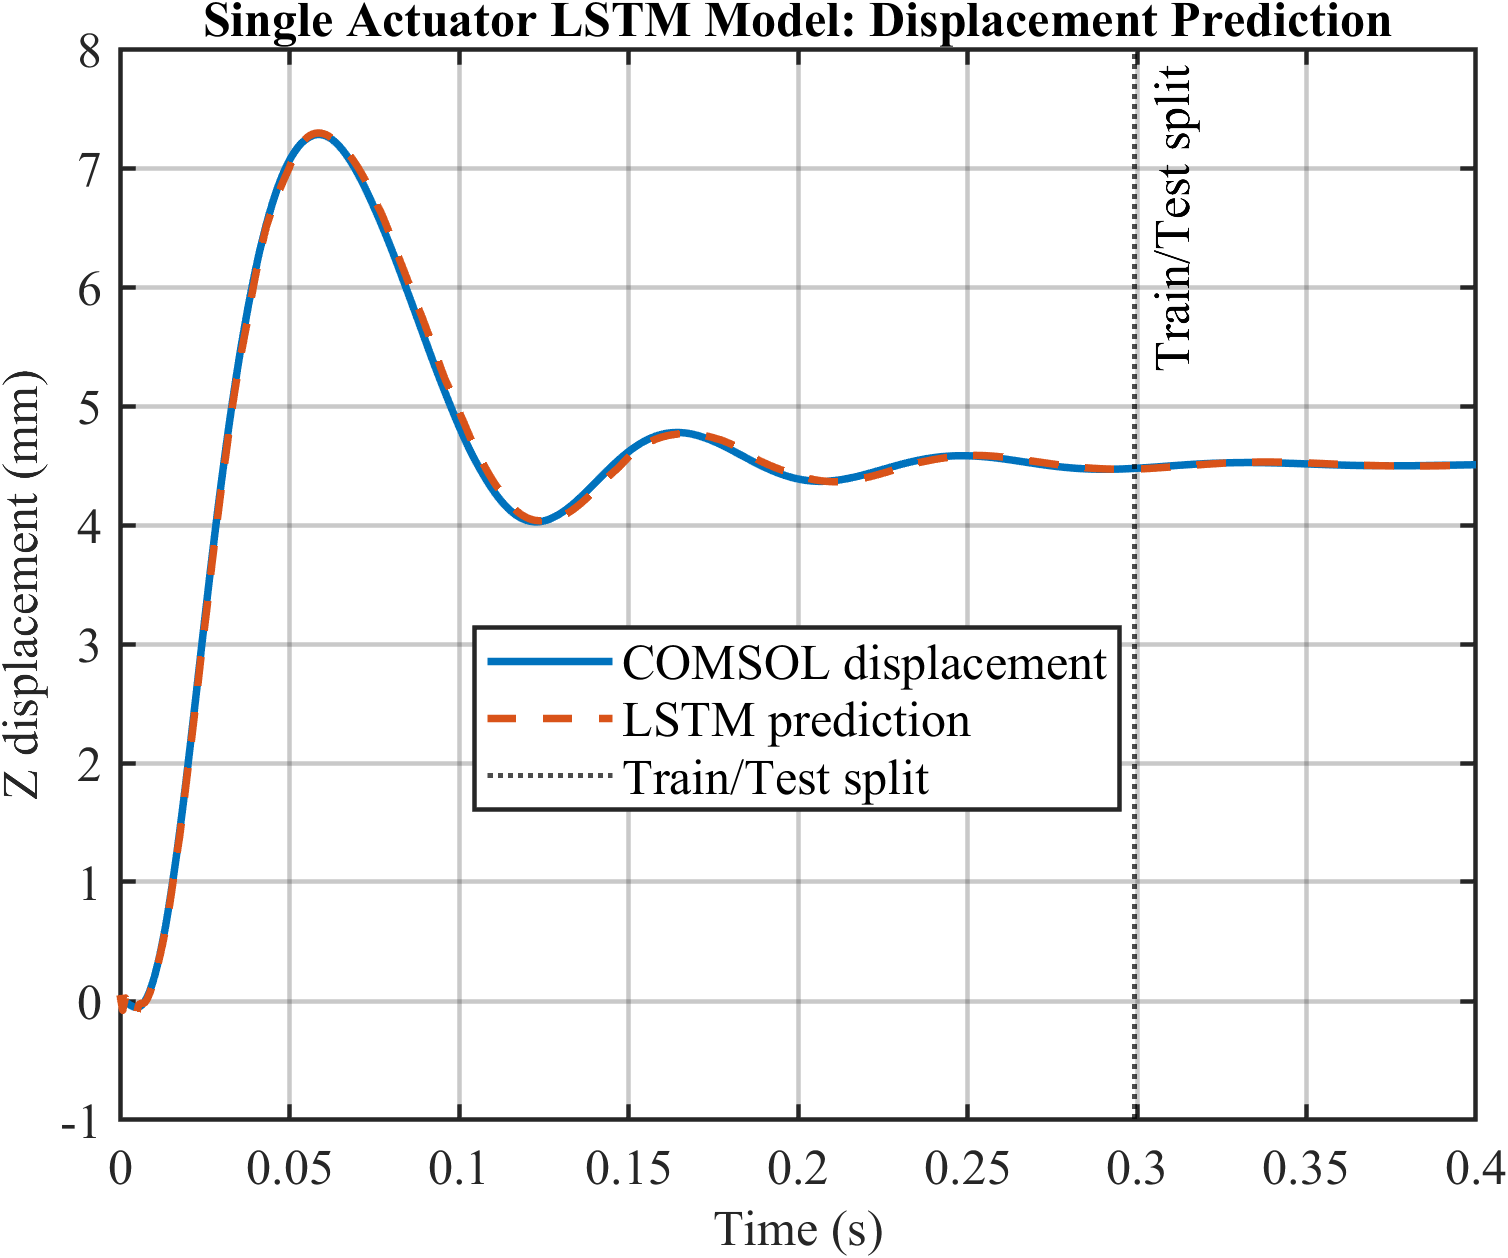
\includegraphics[width=0.92\textwidth]{figures/Fig11_LSTM_Displacement_Prediction.png}
    \caption{Fig11 LSTM Displacement Prediction.}
    \label{fig:fig11_lstm_displacement_prediction}
\end{figure}

\begin{figure}[H]
    \centering
    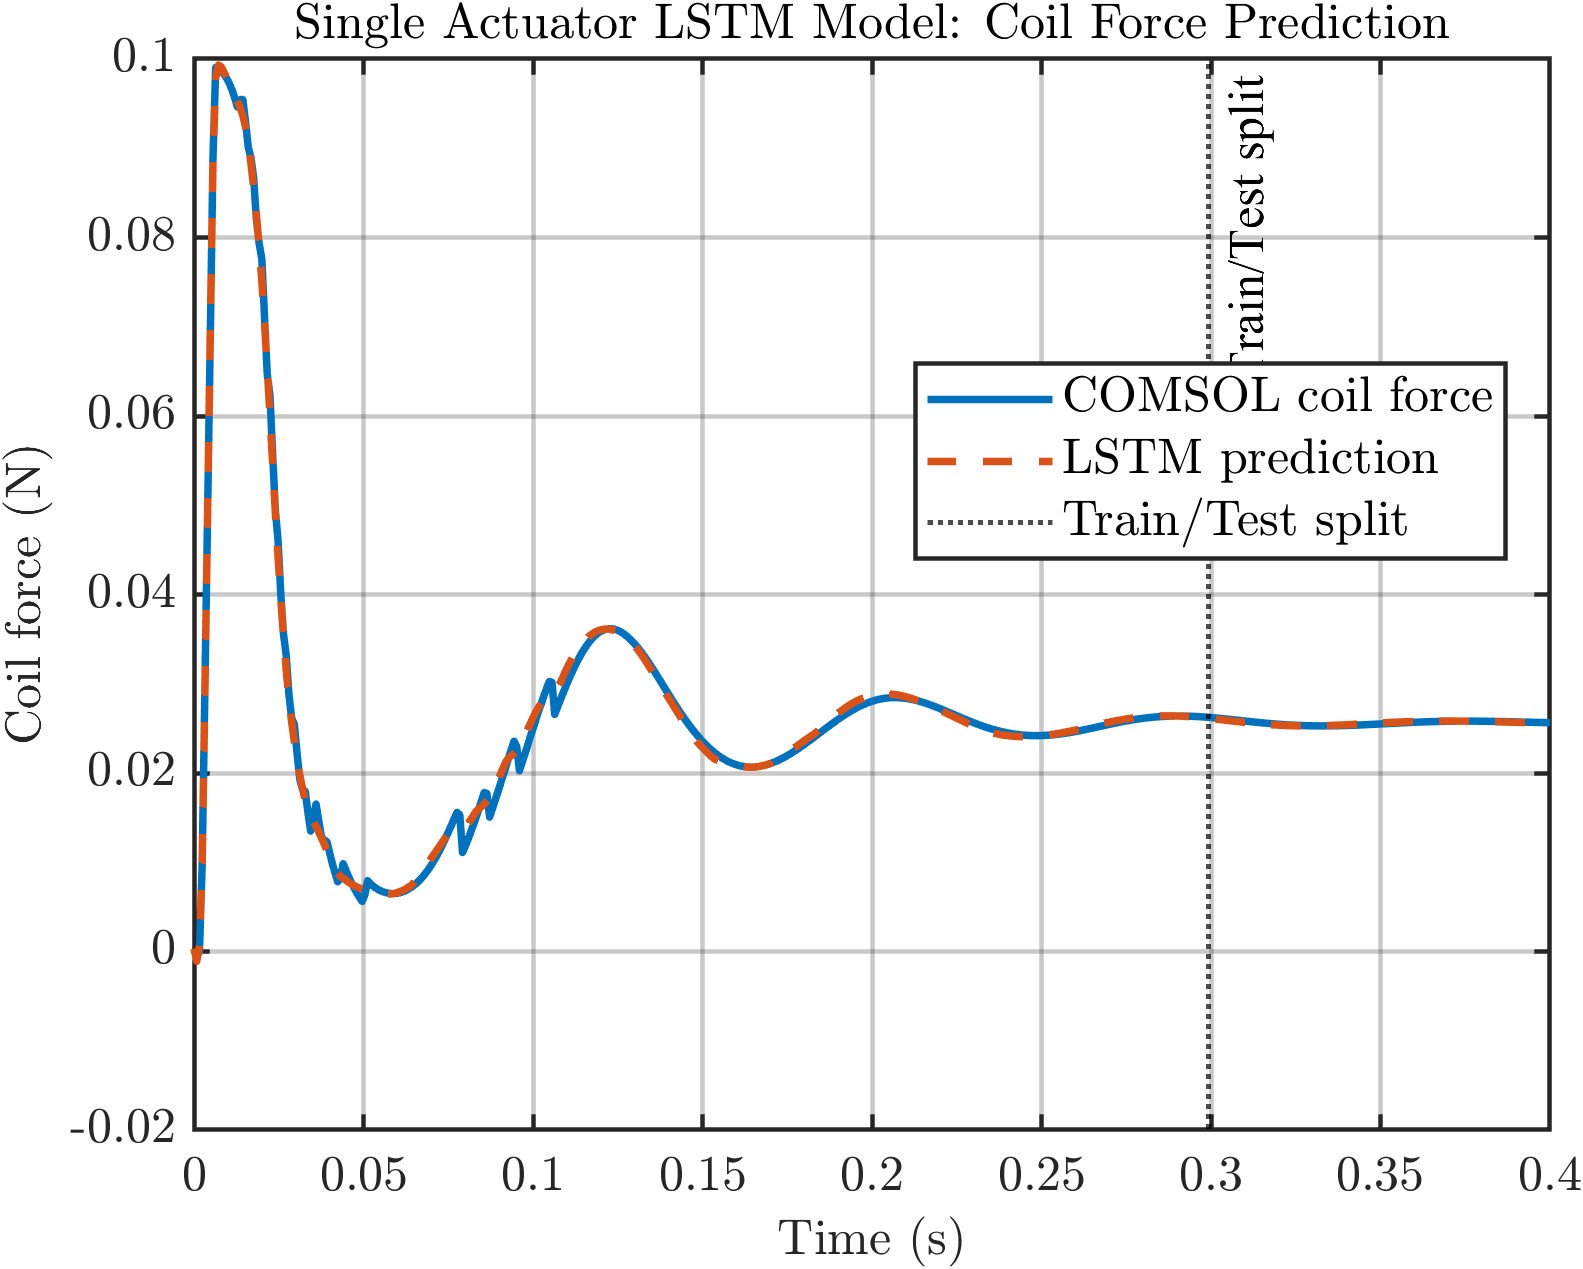
\includegraphics[width=0.92\textwidth]{figures/Fig12_LSTM_Force_Prediction.png}
    \caption{Fig12 LSTM Force Prediction.}
    \label{fig:fig12_lstm_force_prediction}
\end{figure}

\begin{figure}[H]
    \centering
    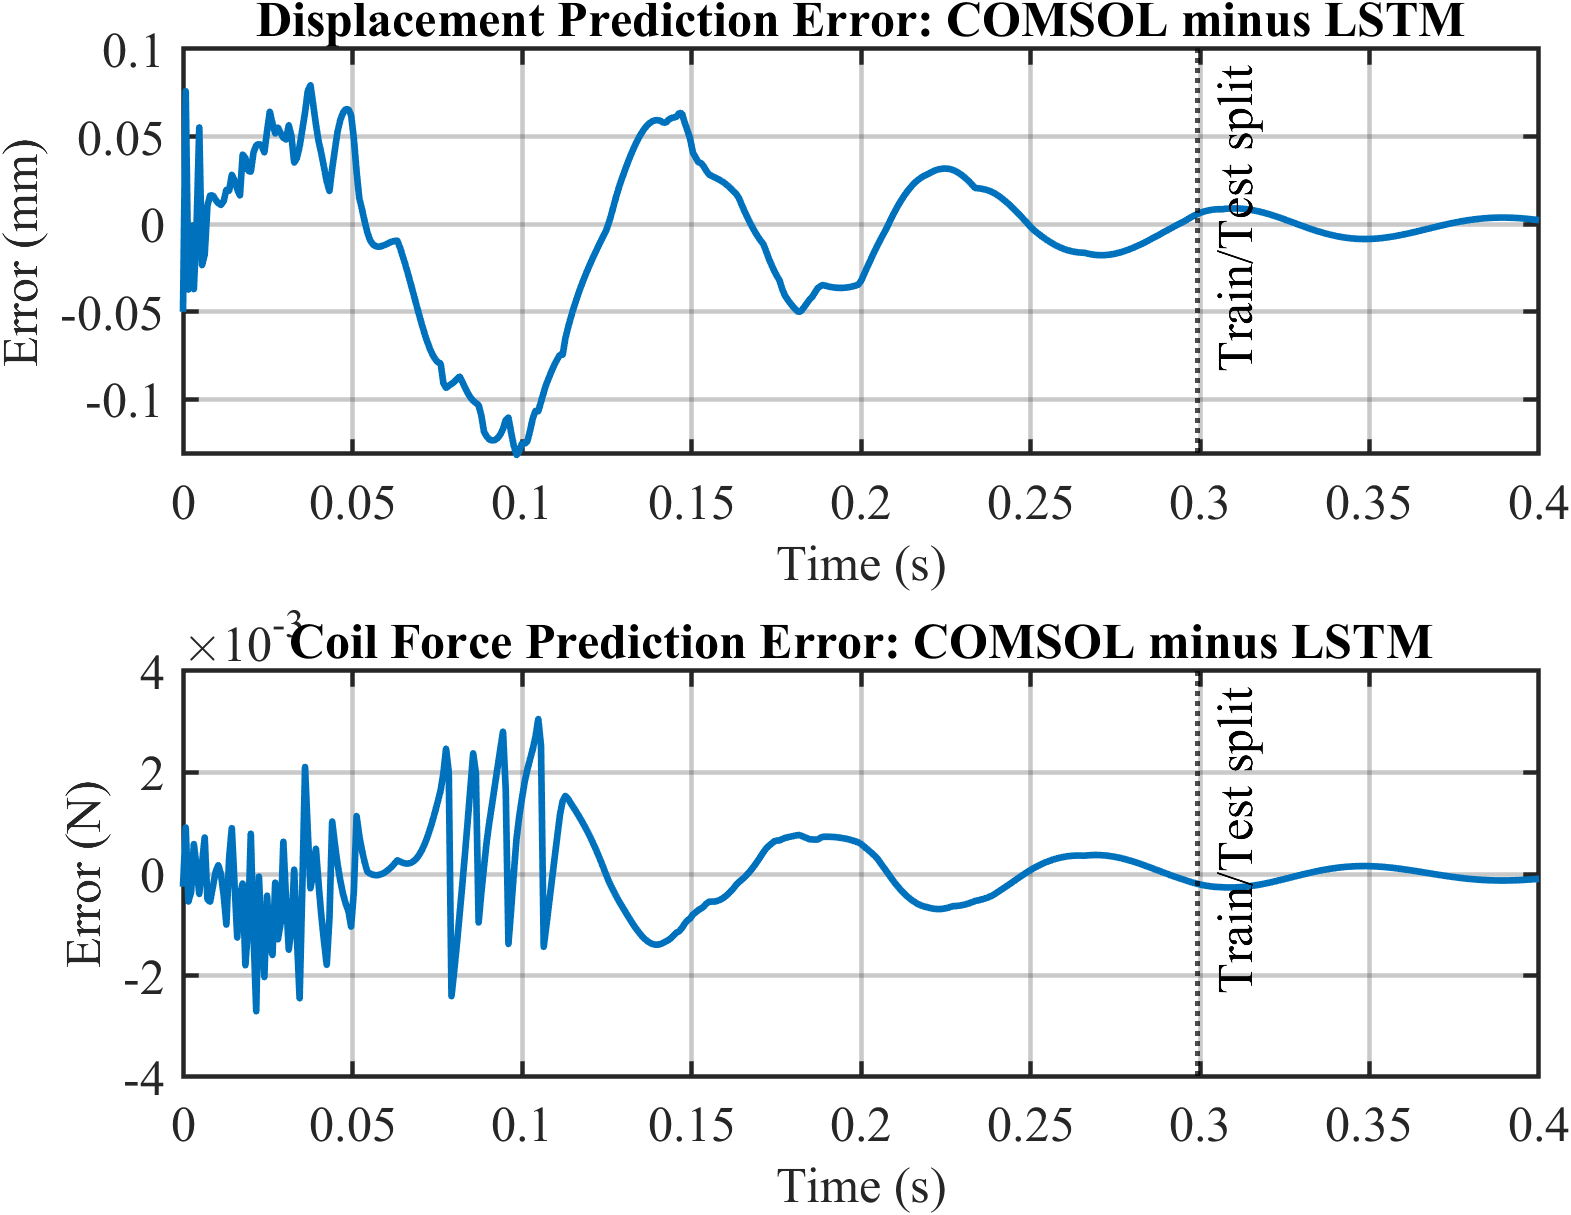
\includegraphics[width=0.92\textwidth]{figures/Fig13_LSTM_Prediction_Errors.png}
    \caption{Fig13 LSTM Prediction Errors.}
    \label{fig:fig13_lstm_prediction_errors}
\end{figure}

\begin{figure}[H]
    \centering
    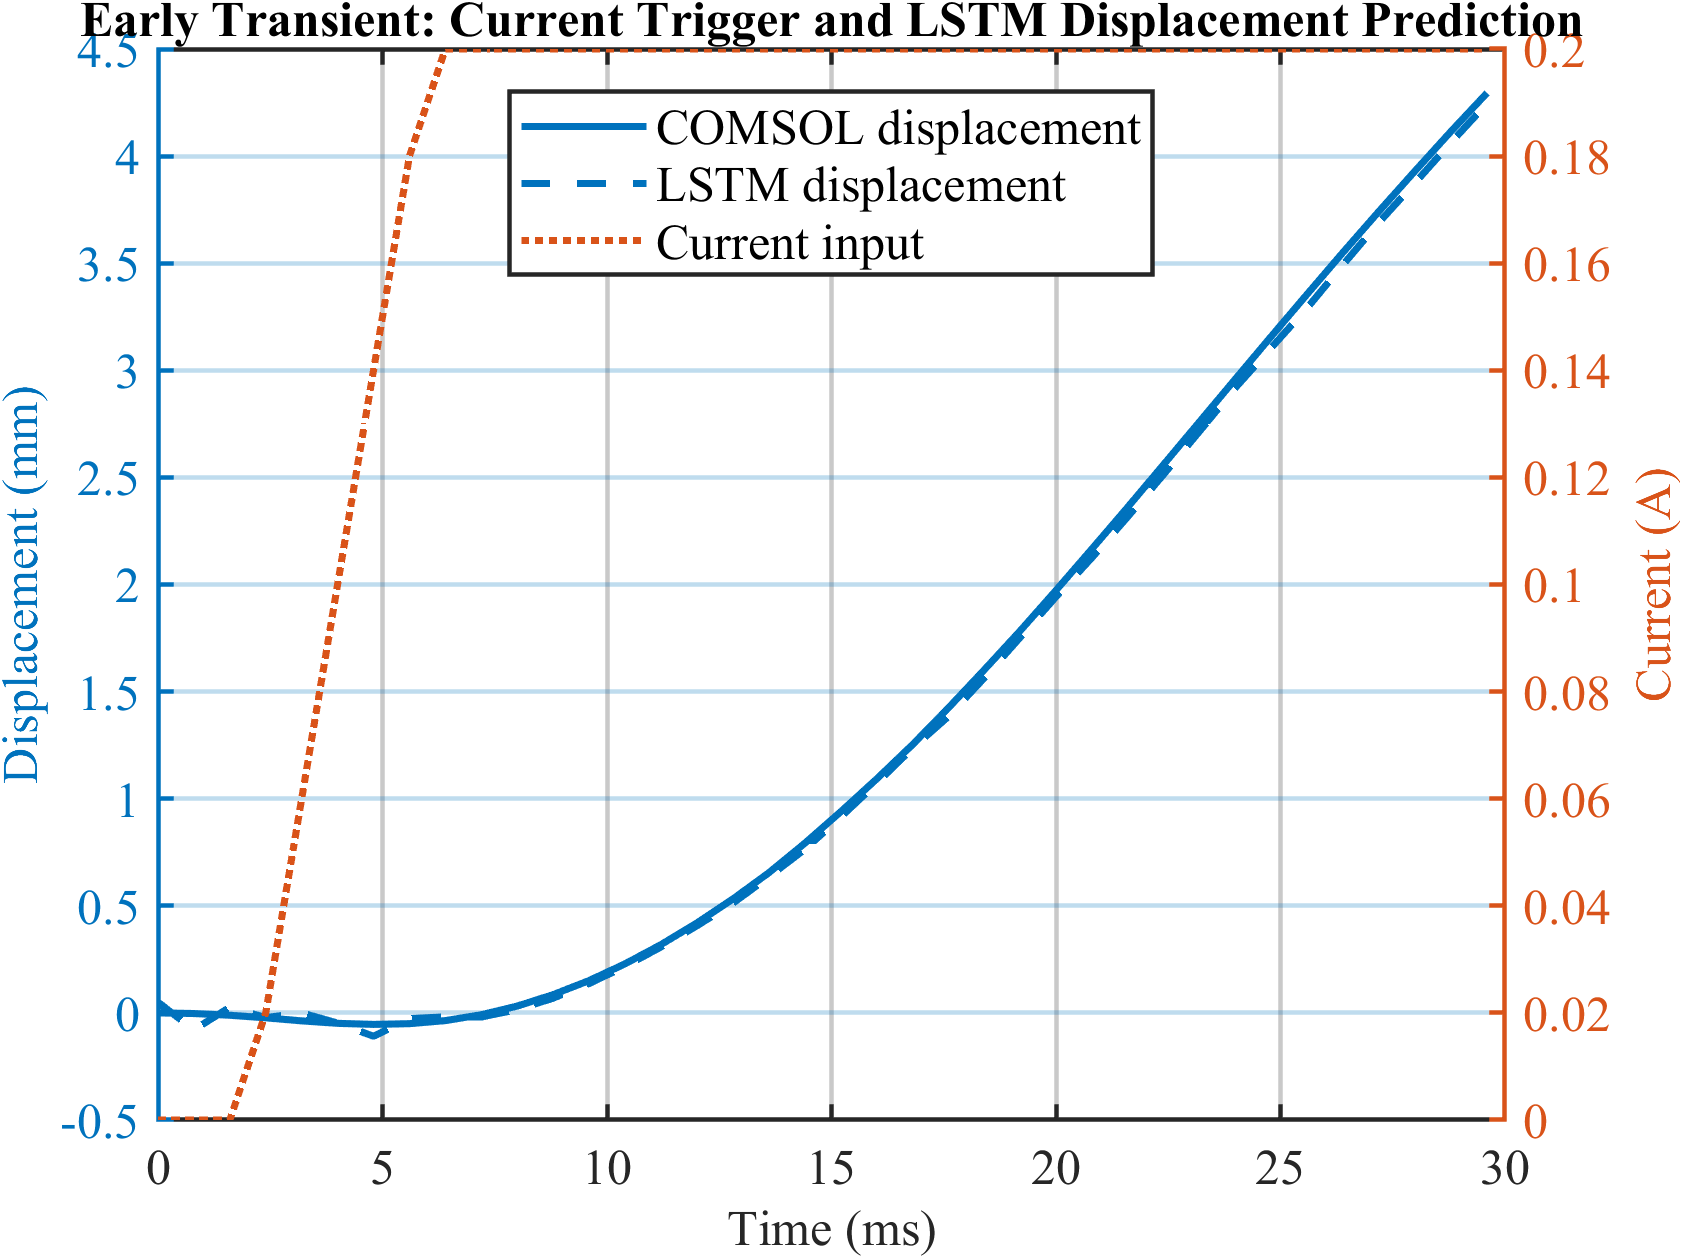
\includegraphics[width=0.92\textwidth]{figures/Fig14_LSTM_TriggerZoom.png}
    \caption{Fig14 LSTM TriggerZoom.}
    \label{fig:fig14_lstm_triggerzoom}
\end{figure}

\begin{figure}[H]
    \centering
    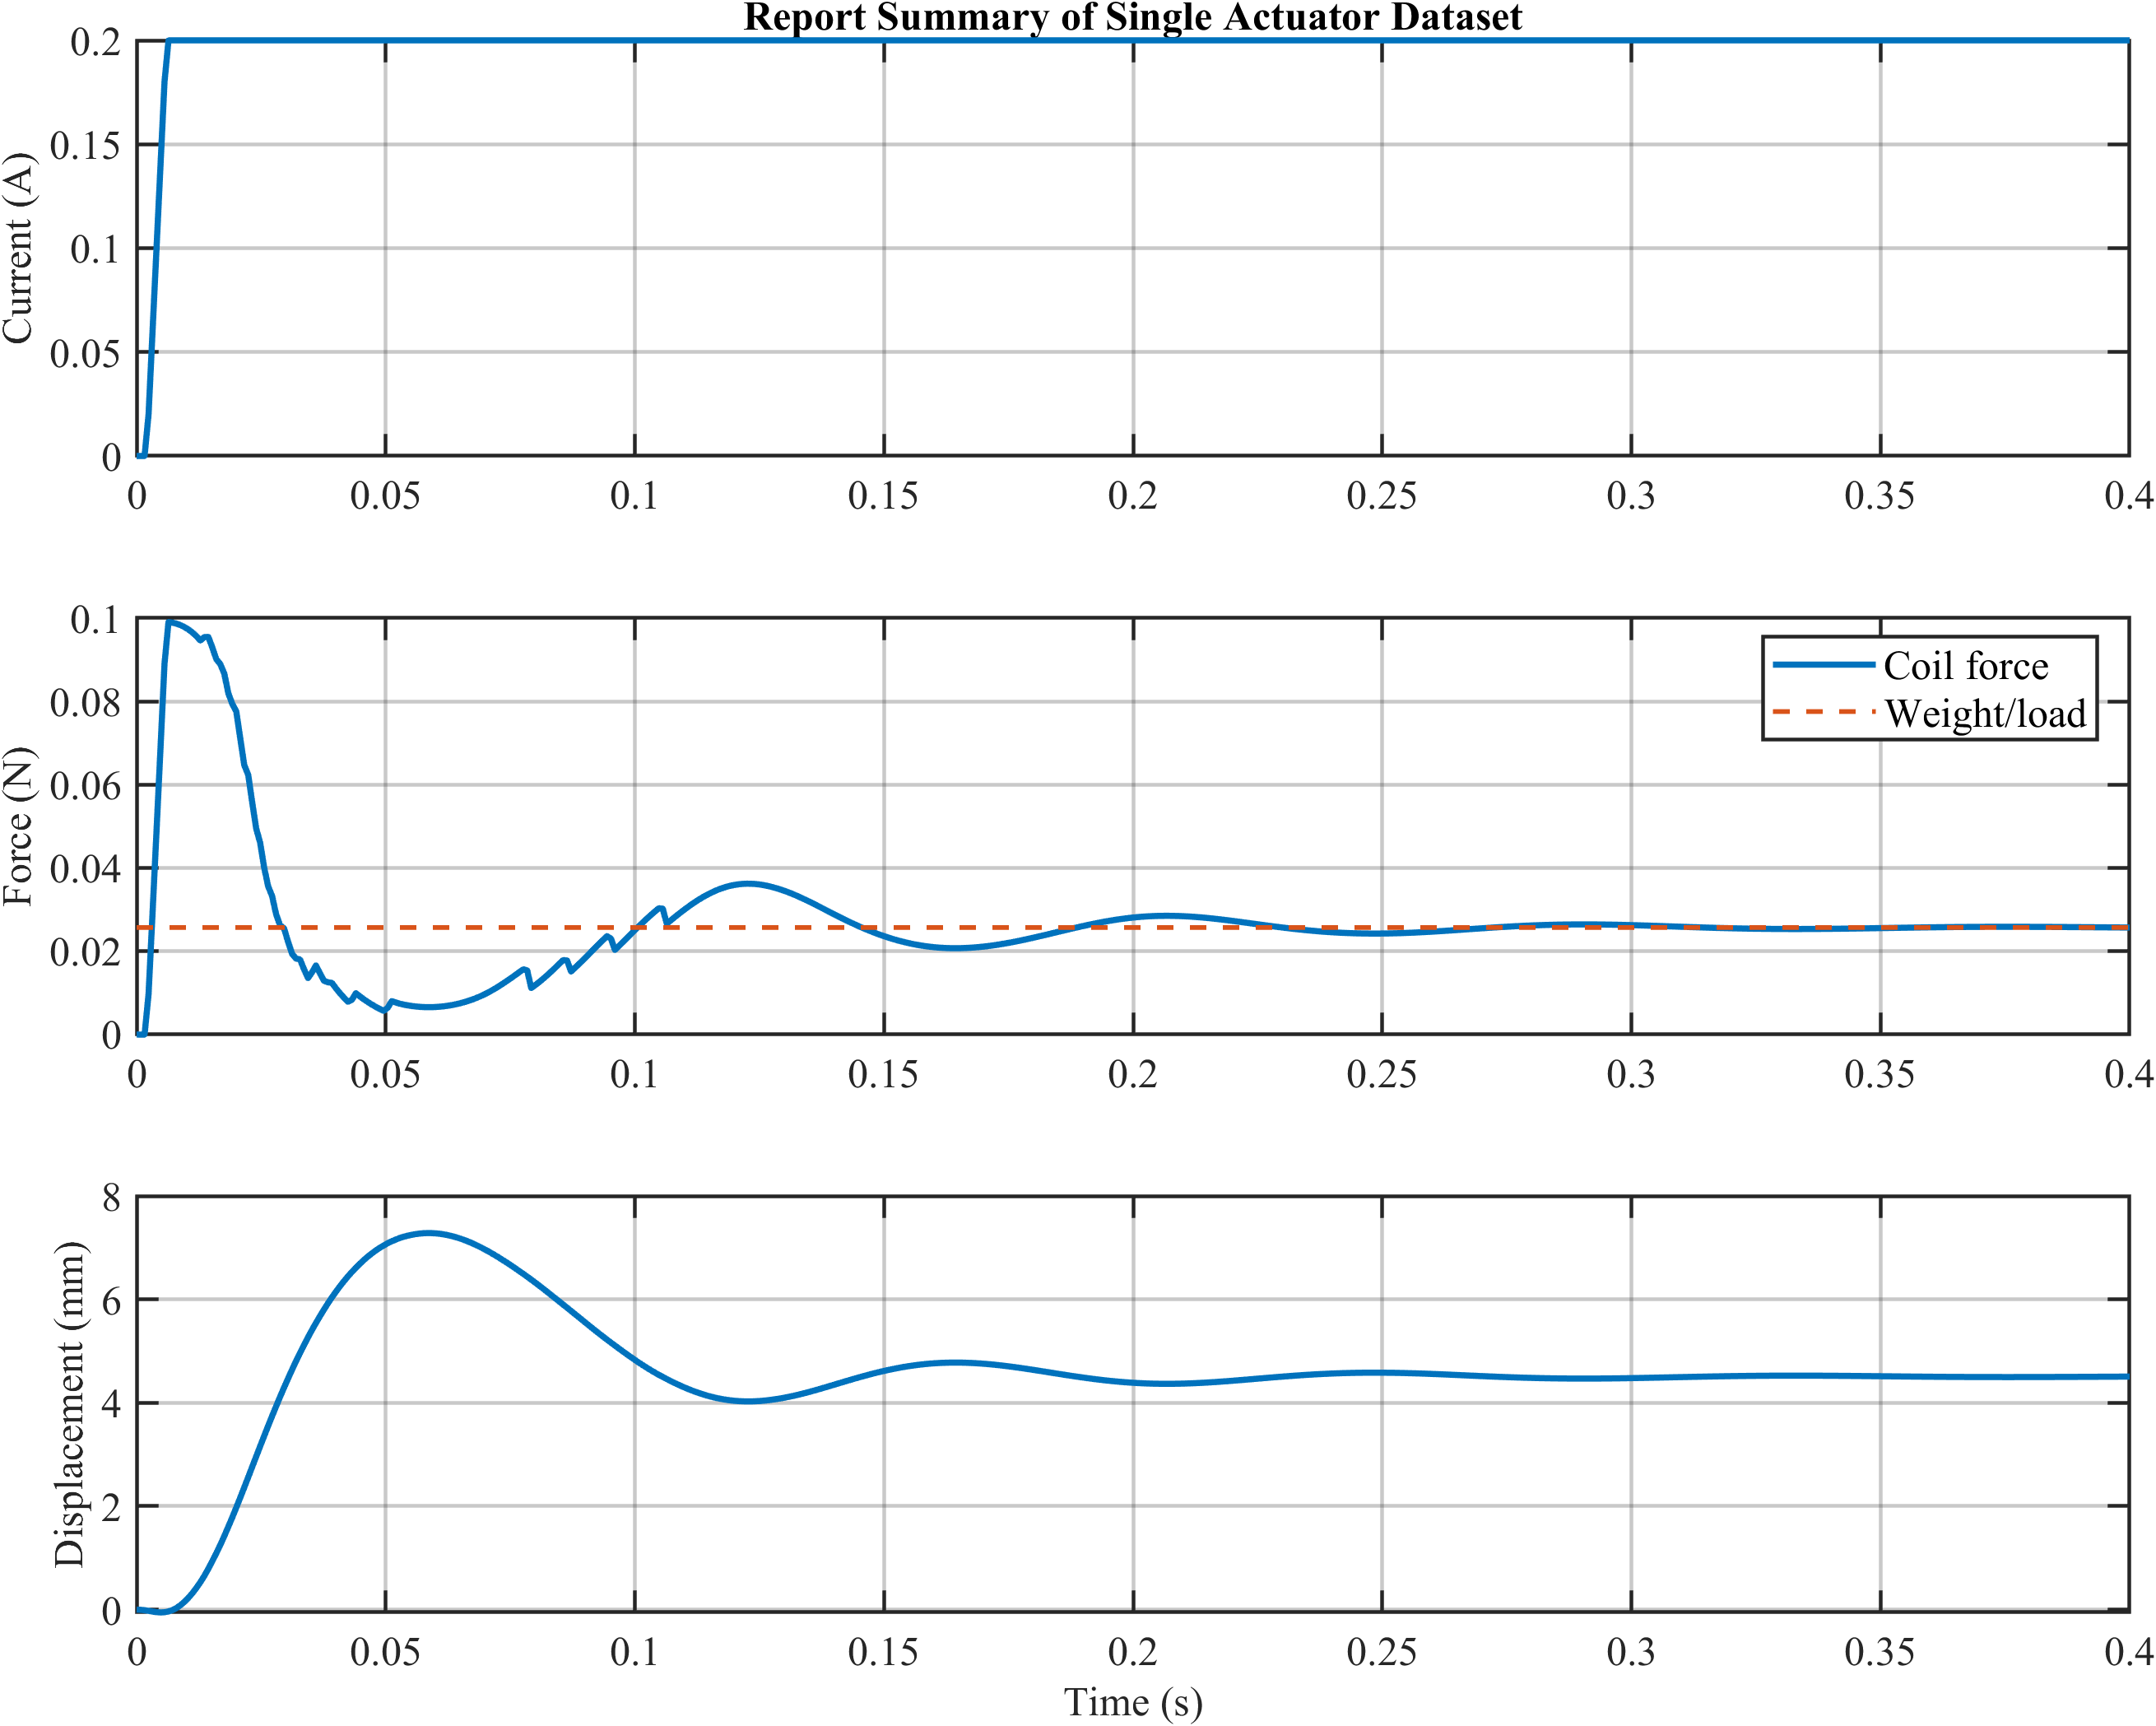
\includegraphics[width=0.92\textwidth]{figures/Fig15_Report_Data_Summary.png}
    \caption{Fig15 Report Data Summary.}
    \label{fig:fig15_report_data_summary}
\end{figure}

\begin{figure}[H]
    \centering
    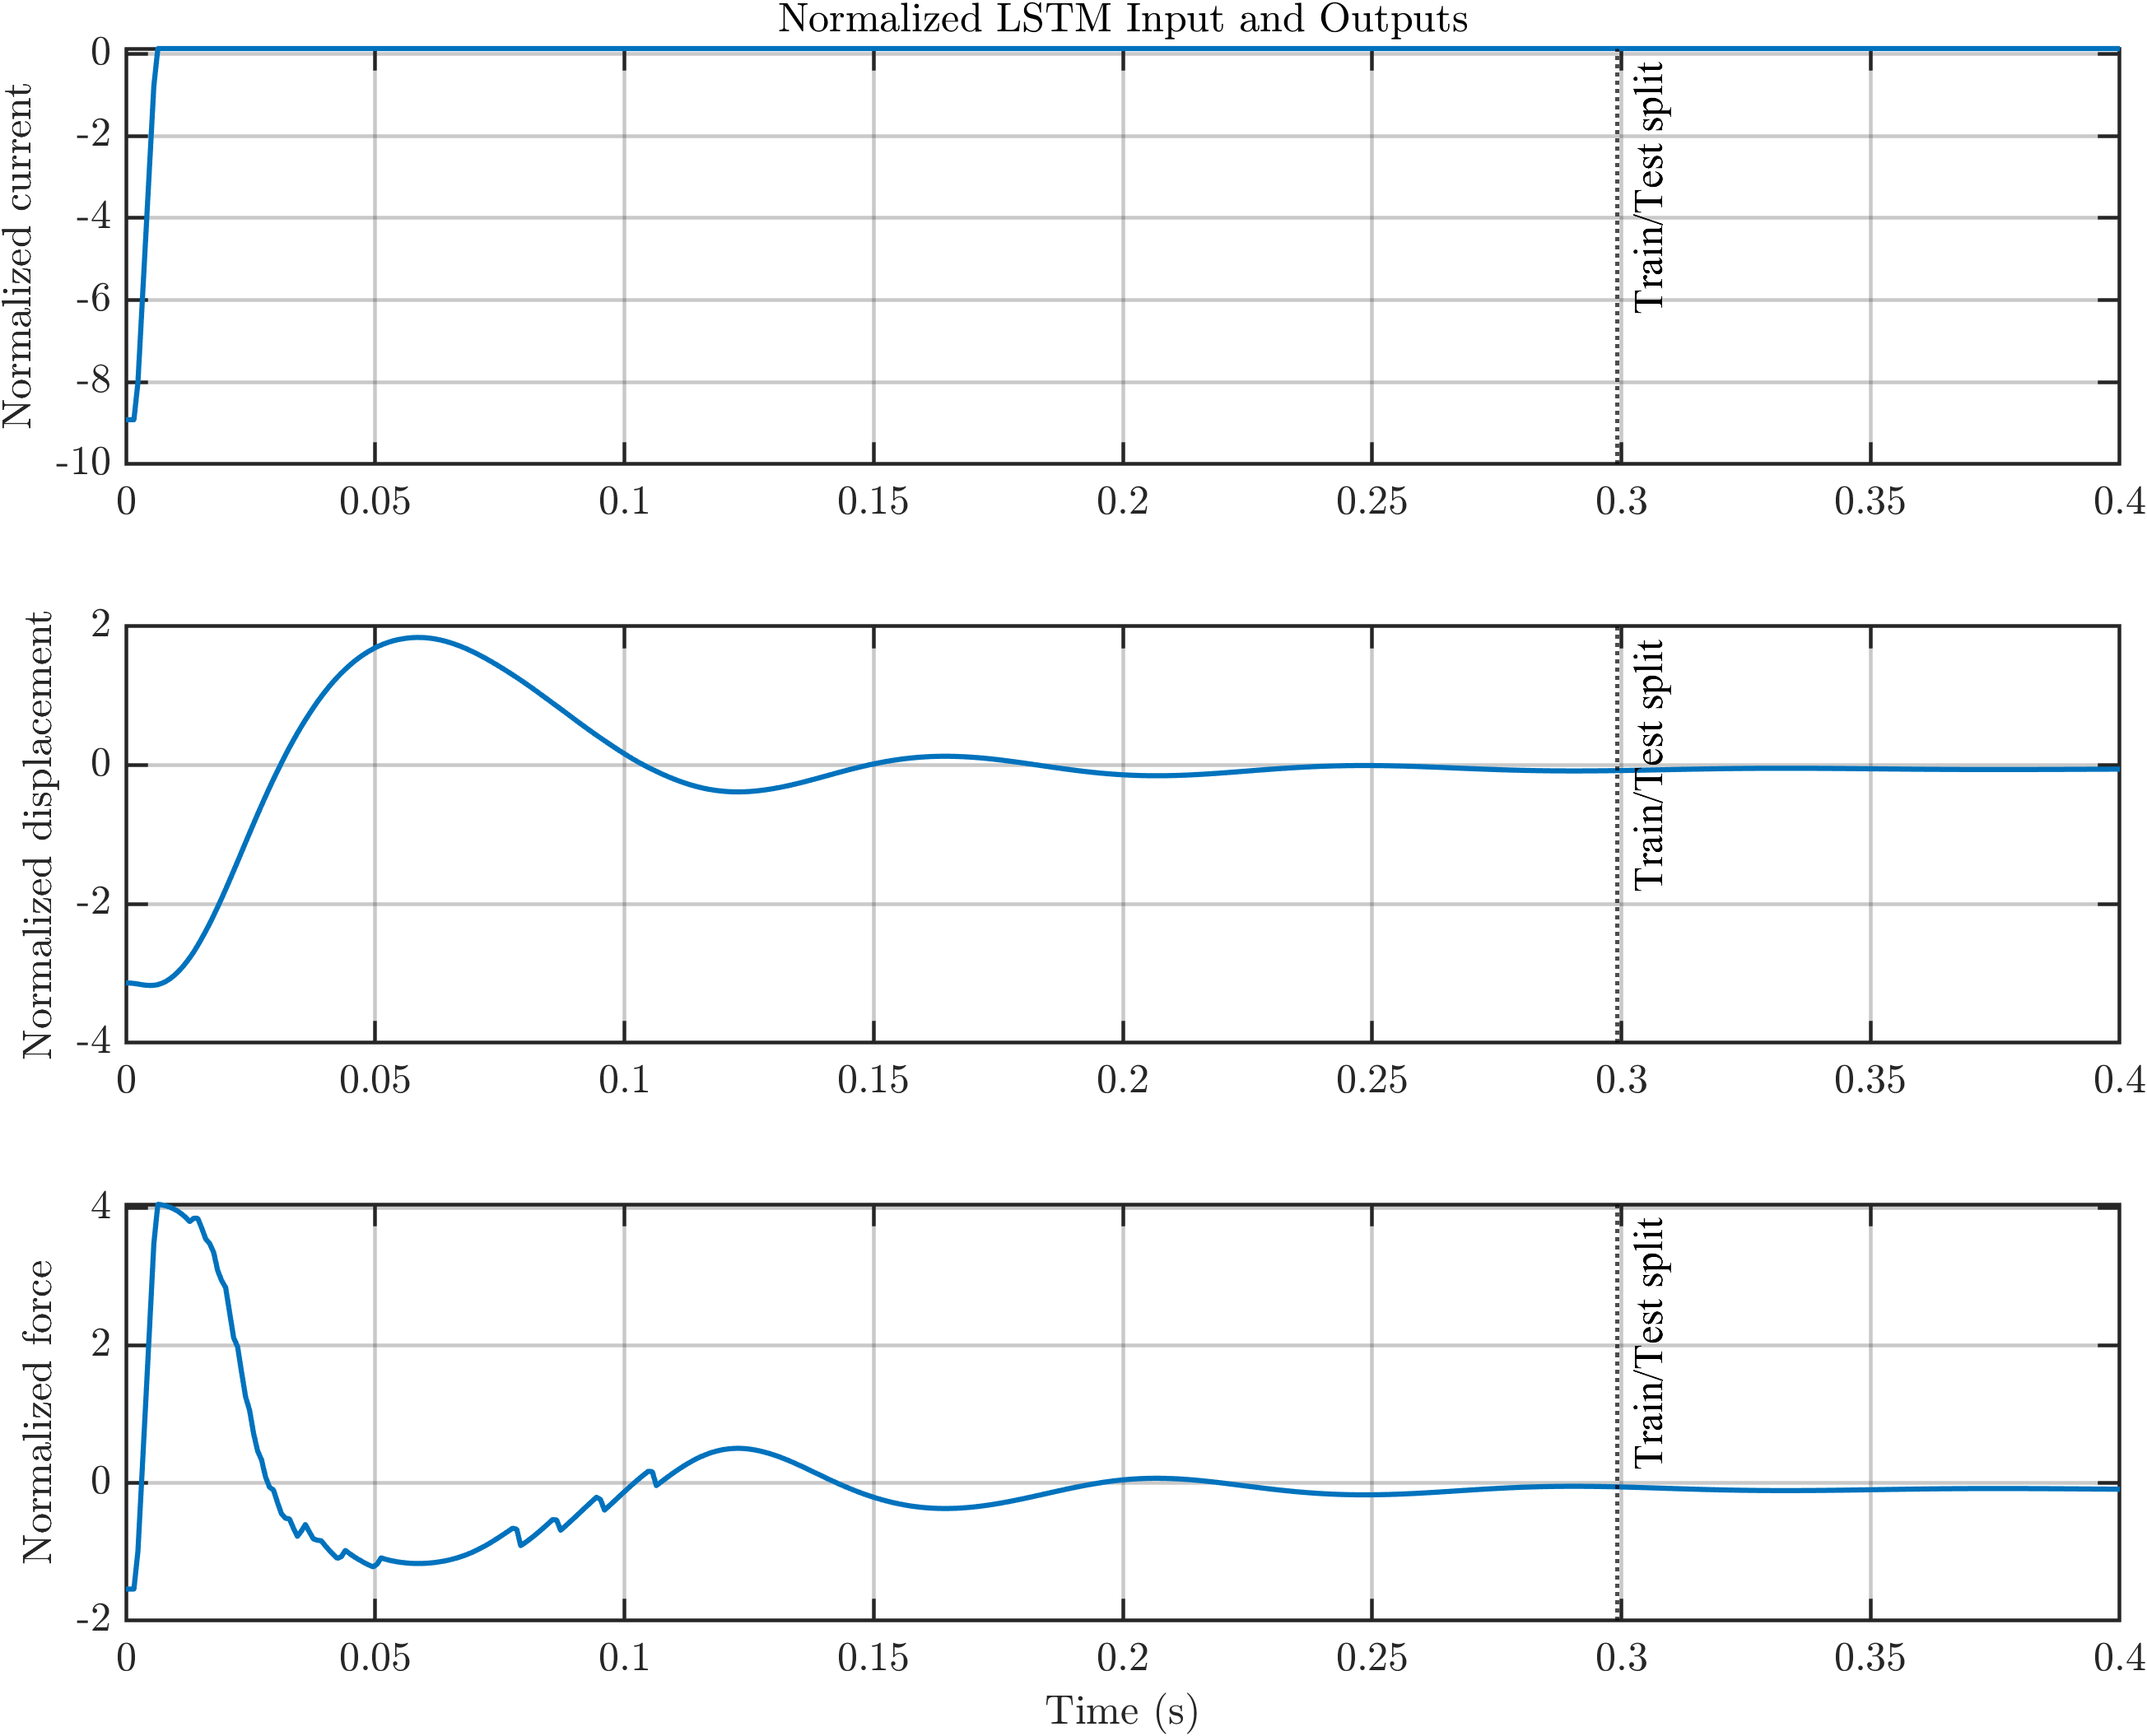
\includegraphics[width=0.92\textwidth]{figures/Fig16_LSTM_Normalized_Sequences.png}
    \caption{Fig16 LSTM Normalized Sequences.}
    \label{fig:fig16_lstm_normalized_sequences}
\end{figure}

\begin{figure}[H]
    \centering
    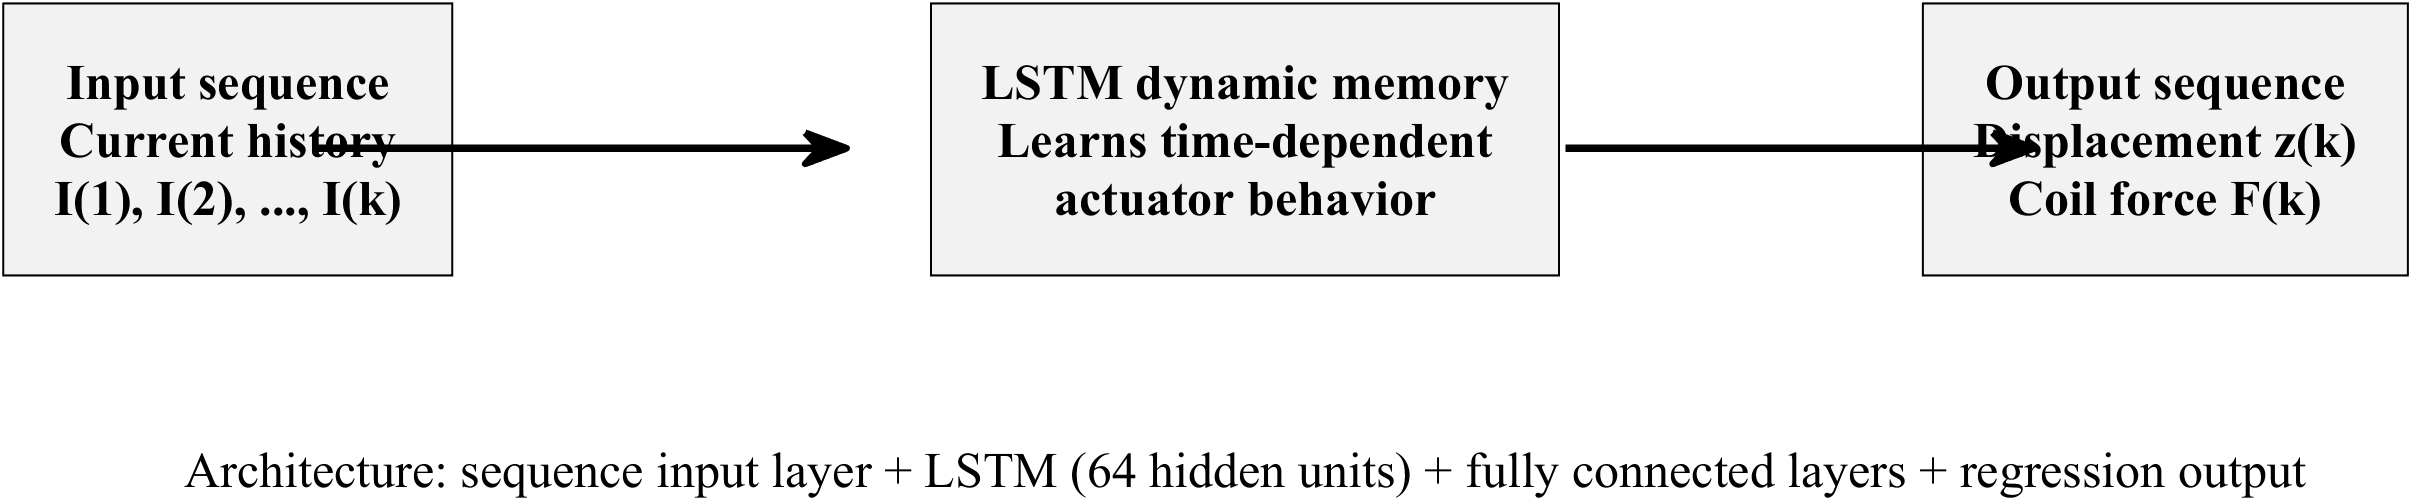
\includegraphics[width=0.92\textwidth]{figures/Fig17_LSTM_Model_Workflow.png}
    \caption{Fig17 LSTM Model Workflow.}
    \label{fig:fig17_lstm_model_workflow}
\end{figure}

\begin{figure}[H]
    \centering
    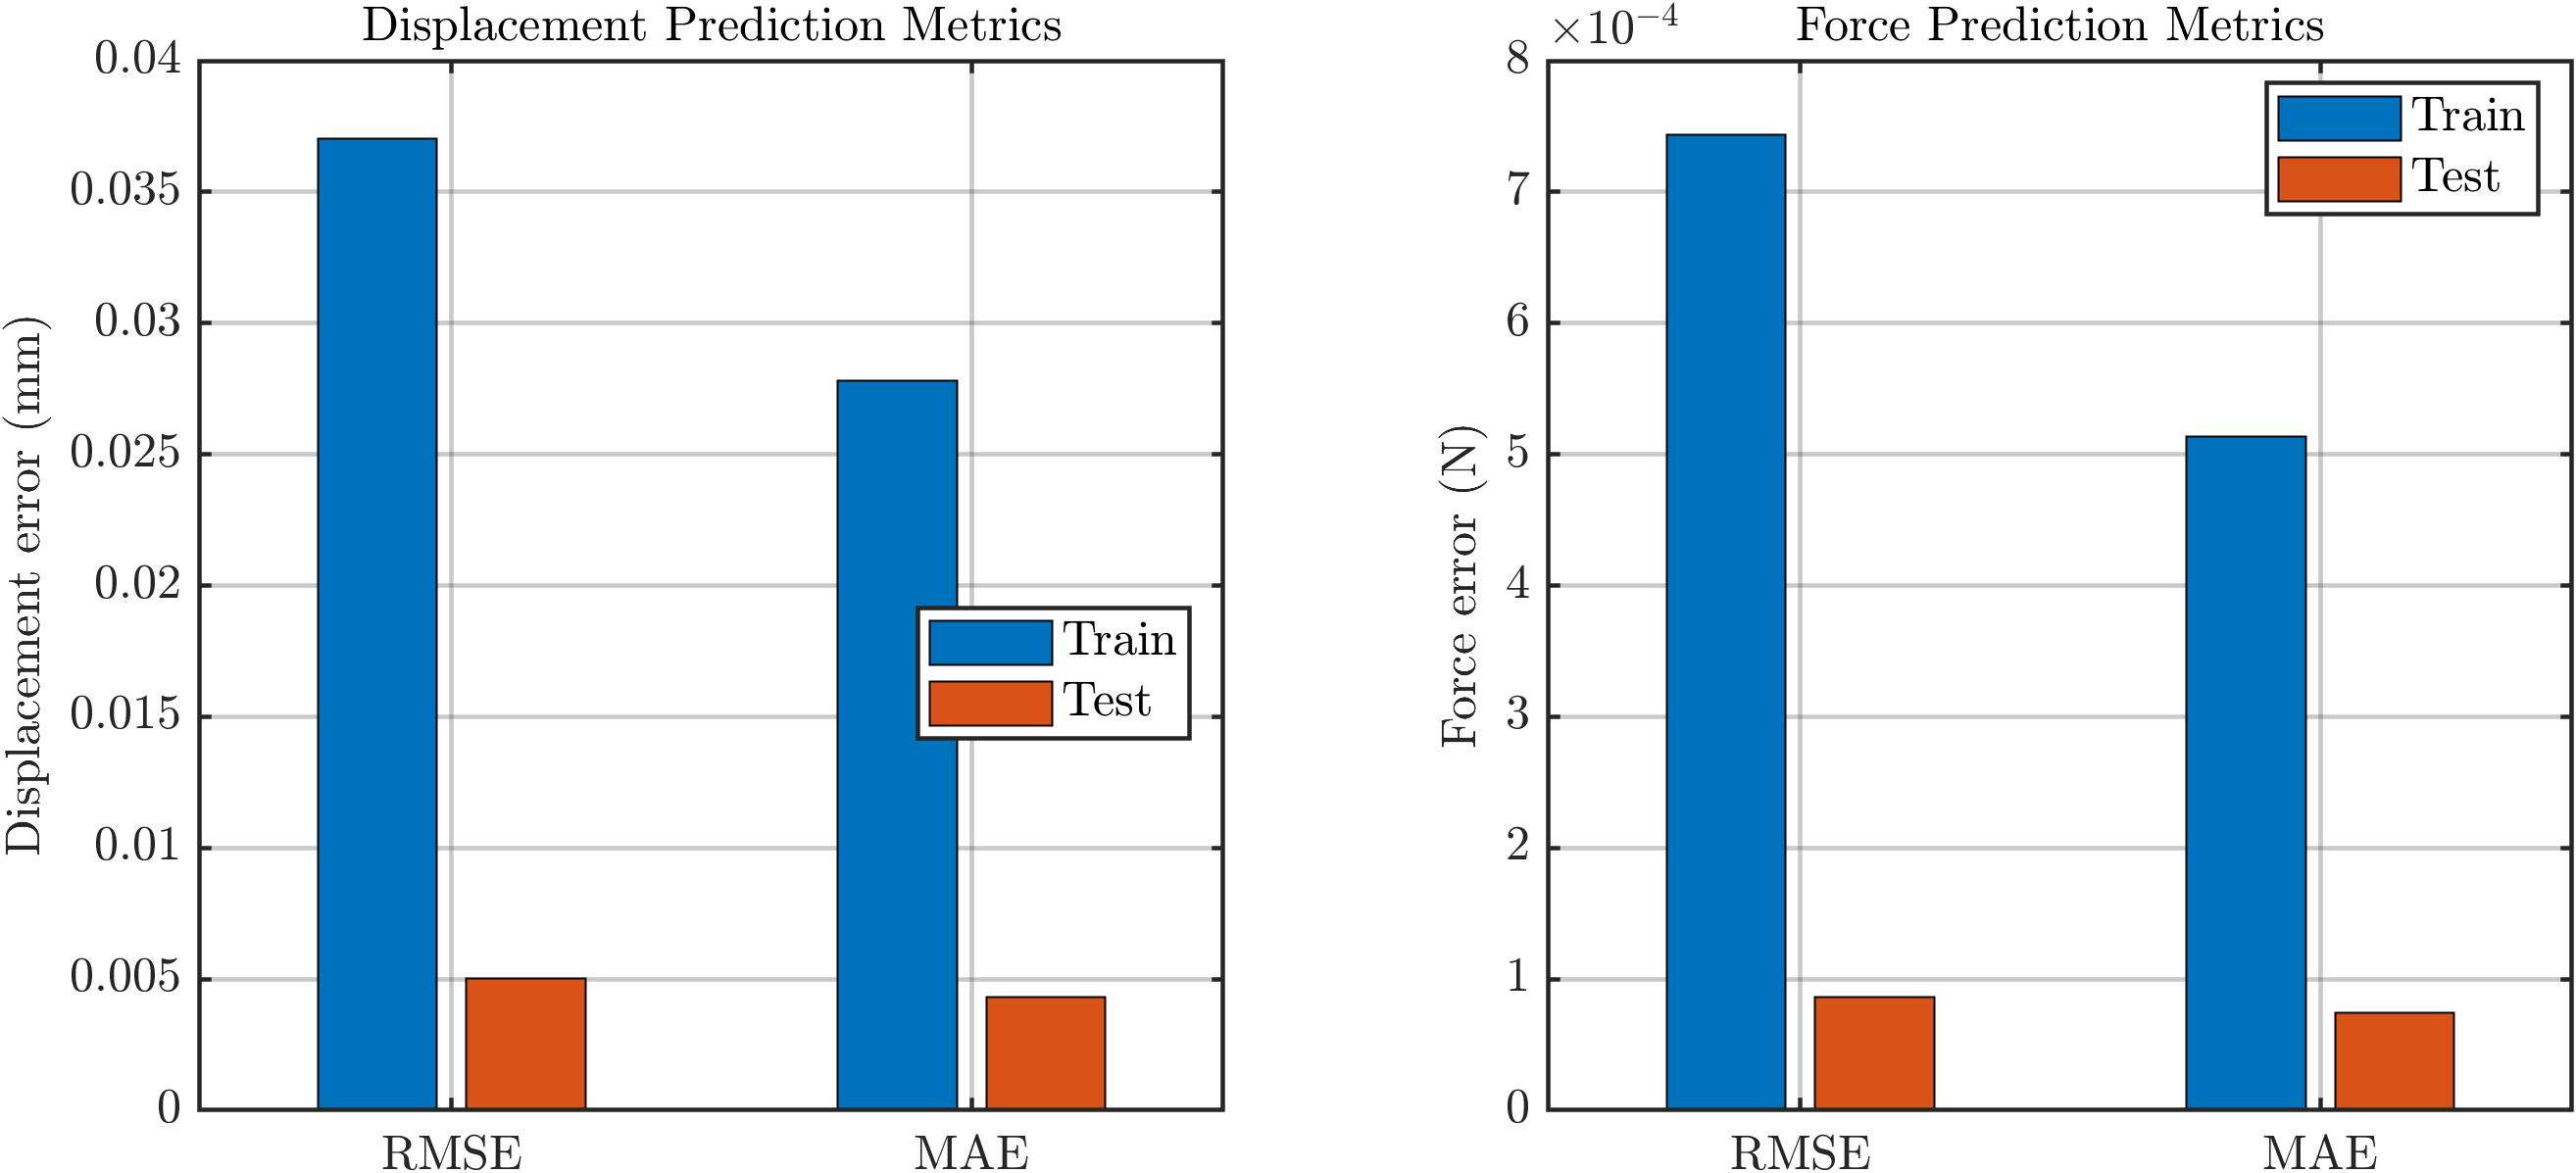
\includegraphics[width=0.92\textwidth]{figures/Fig18_LSTM_Error_Metrics.png}
    \caption{Fig18 LSTM Error Metrics.}
    \label{fig:fig18_lstm_error_metrics}
\end{figure}

\begin{figure}[H]
    \centering
    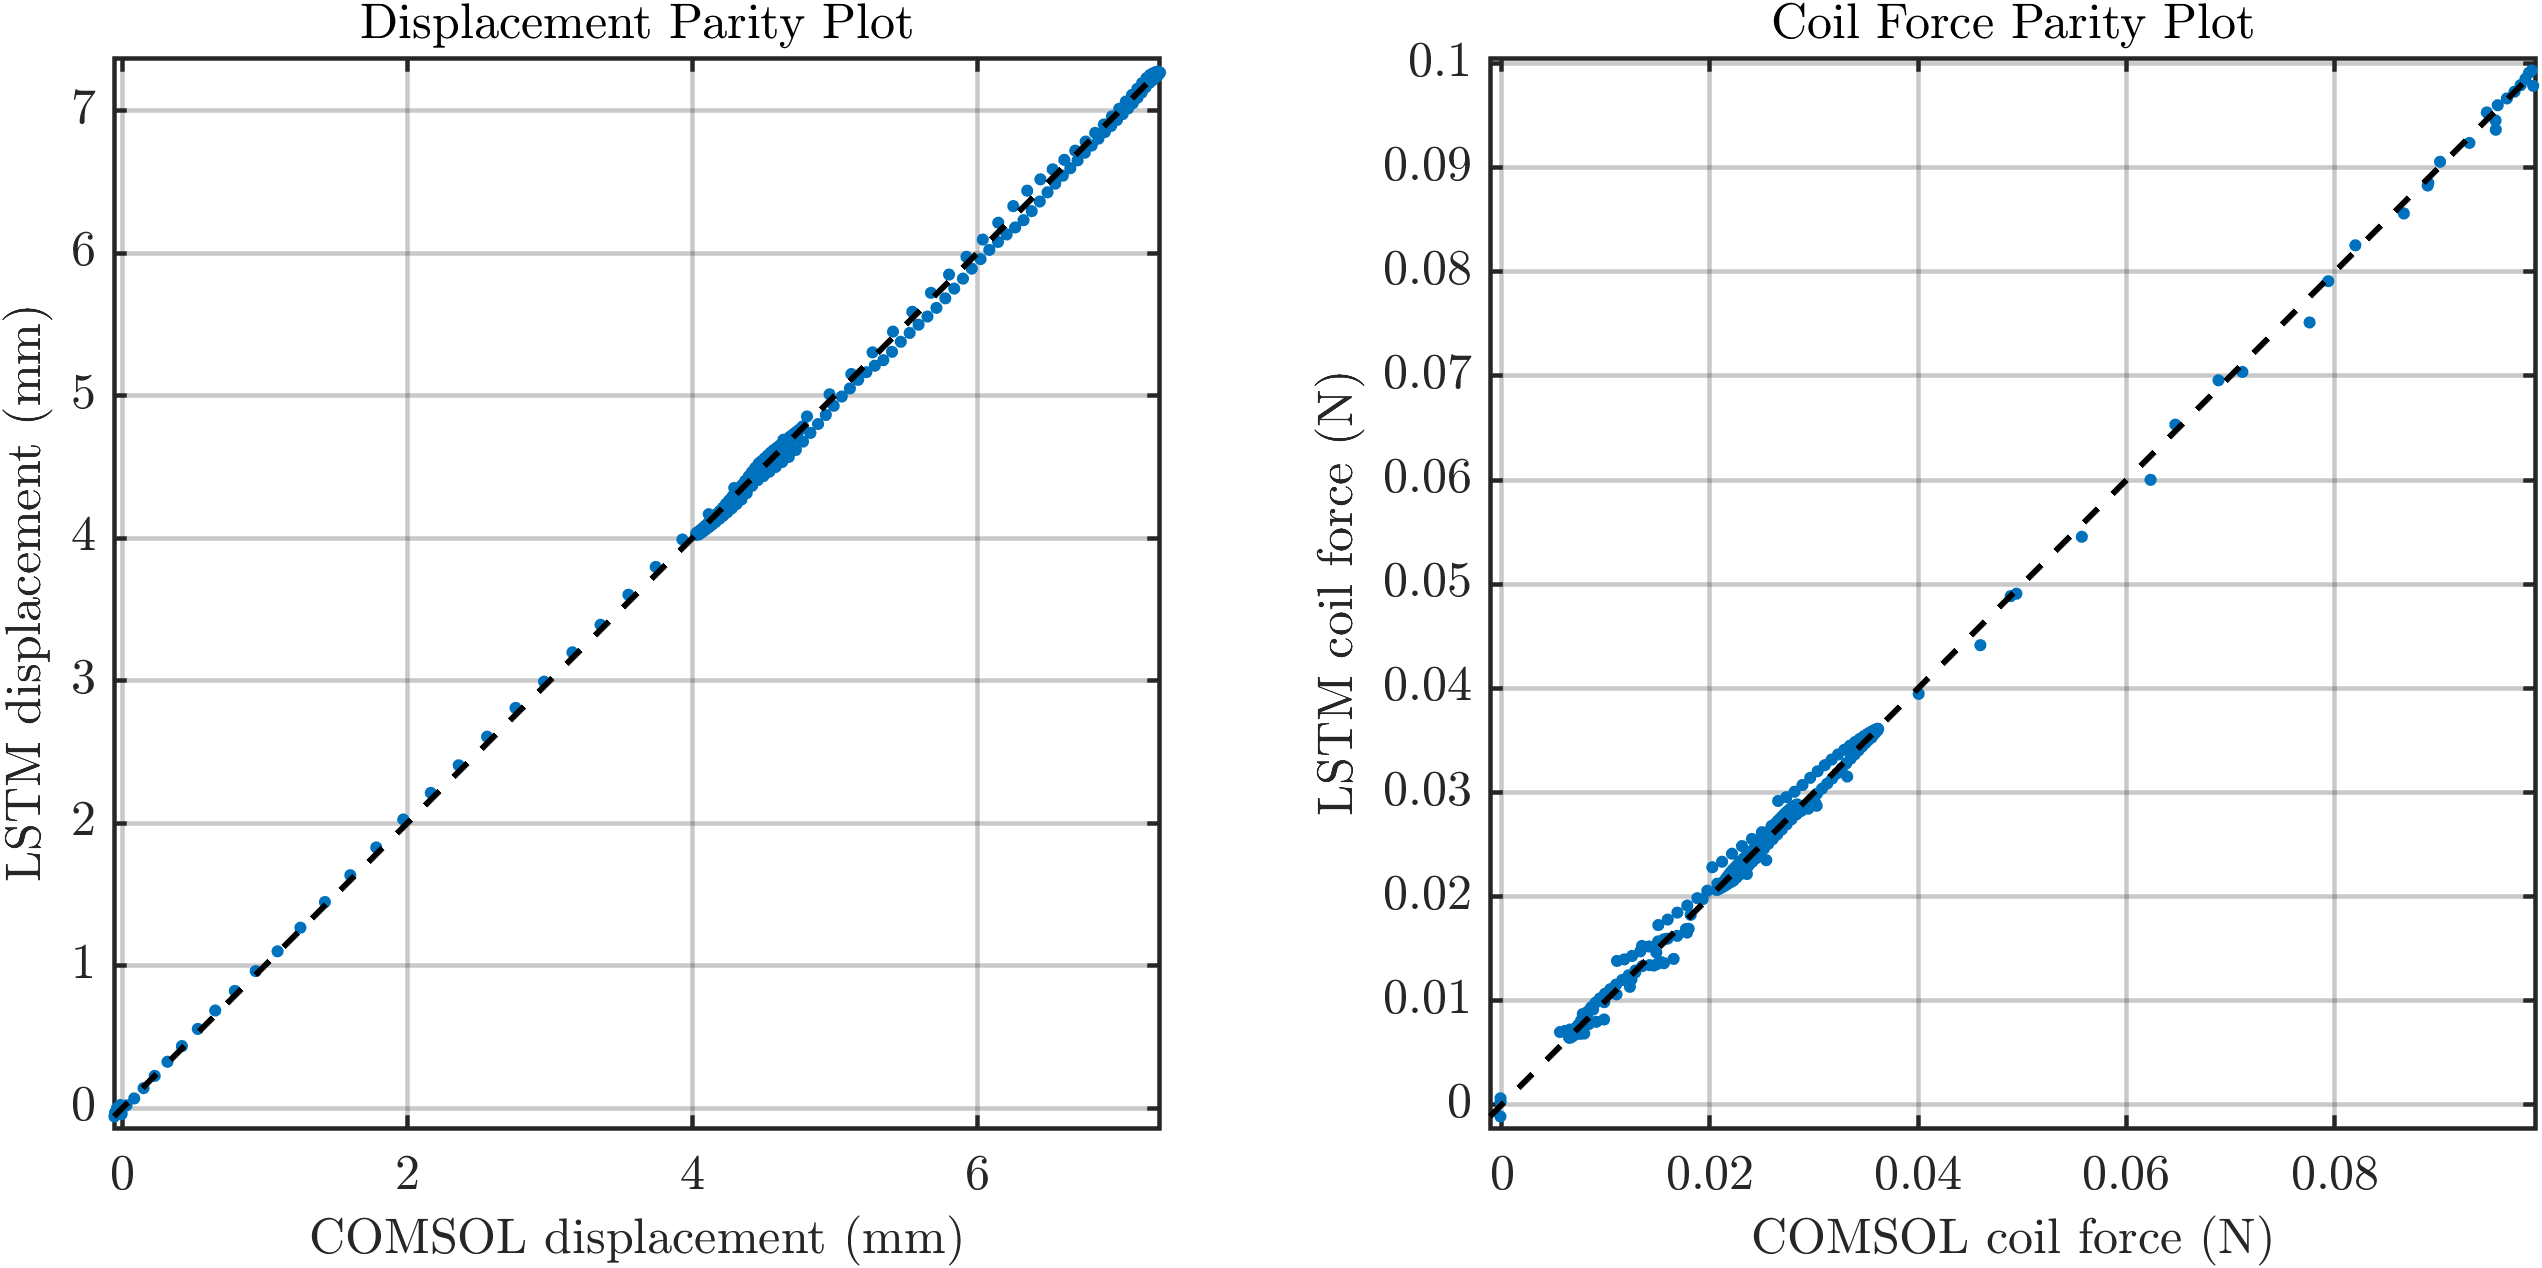
\includegraphics[width=0.92\textwidth]{figures/Fig19_LSTM_Parity_Plots.png}
    \caption{Fig19 LSTM Parity Plots.}
    \label{fig:fig19_lstm_parity_plots}
\end{figure}

\begin{figure}[H]
    \centering
    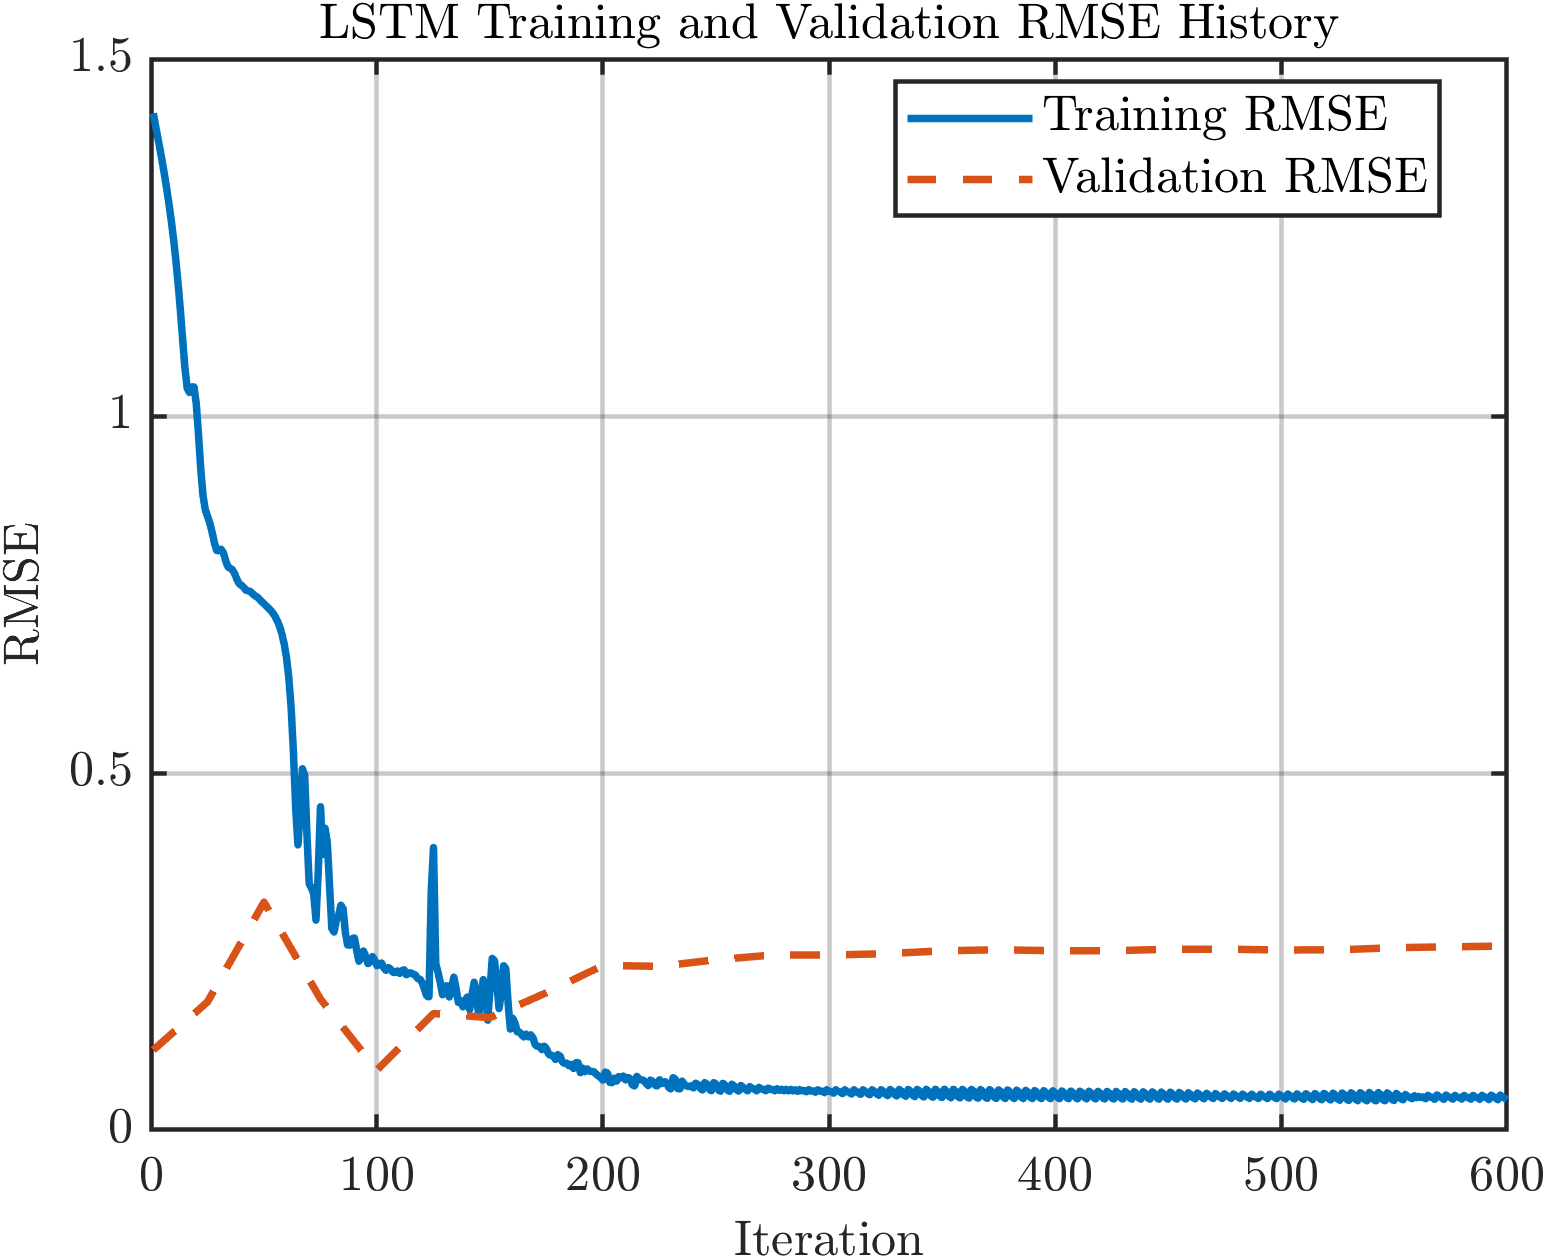
\includegraphics[width=0.92\textwidth]{figures/Fig20_LSTM_Training_RMSE_History.png}
    \caption{Fig20 LSTM Training RMSE History.}
    \label{fig:fig20_lstm_training_rmse_history}
\end{figure}

\begin{figure}[H]
    \centering
    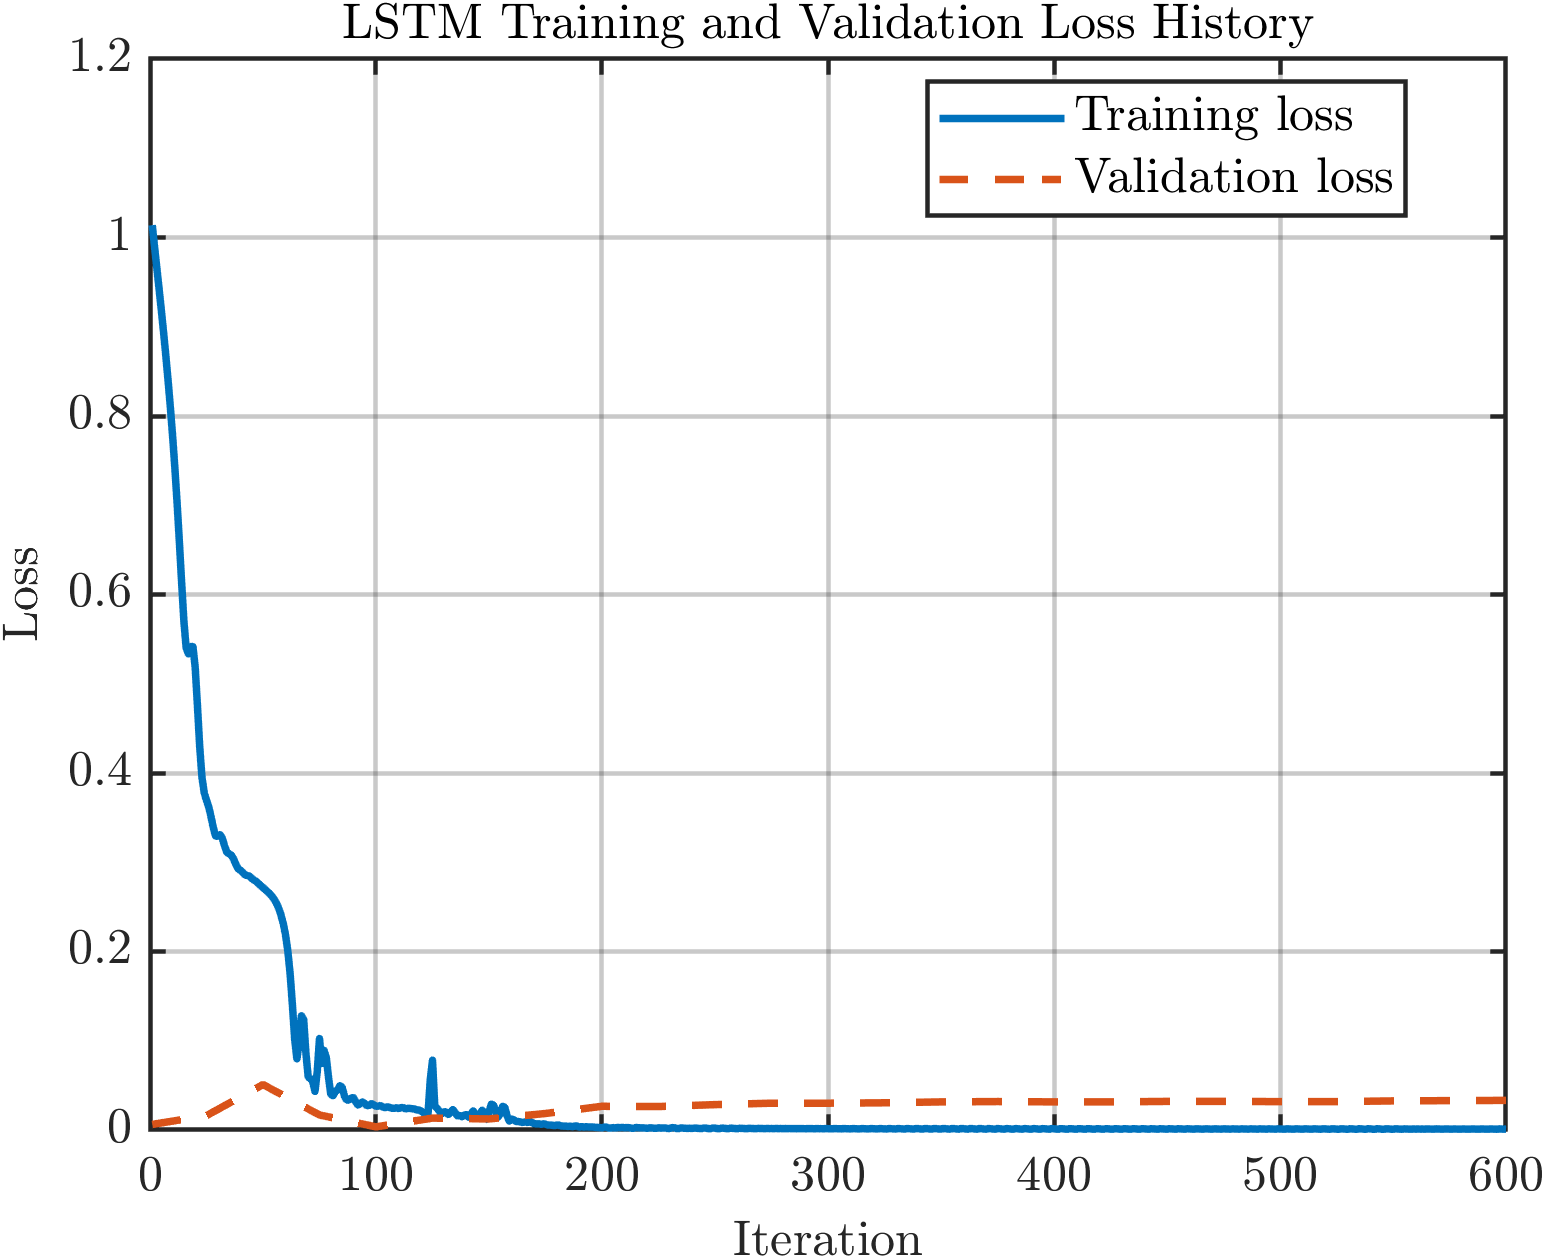
\includegraphics[width=0.92\textwidth]{figures/Fig21_LSTM_Training_Loss_History.png}
    \caption{Fig21 LSTM Training Loss History.}
    \label{fig:fig21_lstm_training_loss_history}
\end{figure}

